\documentclass[a4,11pt]{article}
\usepackage[utf8]{inputenc}
\usepackage[english]{babel}
\usepackage[margin=3cm]{geometry}
\usepackage{tikz}
\usepackage{pgfplots}
\usepackage{pgfplotstable}
\usepackage{biblatex}
\usepackage{amsmath}
\usepackage{amsfonts}
\usepackage{url}
\usepackage{etoolbox}
\usepackage{graphicx}
\usepackage{subcaption}
\usepackage{hyperref}

\usetikzlibrary{positioning,arrows.meta}

\pgfplotsset{
    compat=1.15,
    perf/.style={
        small,
		width=7cm,
		height=3.5cm,
		axis y line=left,
        axis x line=bottom,
        enlarge y limits=0.05,
        enlarge x limits=0.05,
		ymajorgrids=true,
		xmajorgrids=true,
		grid style=dashed,
        xlabel style={
            font=\footnotesize,
            at={(current axis.right of origin)},
            anchor=west
        },
        ylabel style={
            font=\footnotesize,
        },
        title style={
            font=\footnotesize,
        },
    },
    discard if not/.style 2 args={
        x filter/.append code={
            \edef\tempa{\thisrow{#1}}
            \edef\tempb{#2}
            \ifx\tempa\tempb
            \else
                \def\pgfmathresult{inf}
            \fi
        }
    }
}

\makeatletter
\newcommand{\pgfplotsxmin}{\pgfplots@xmin}
\newcommand{\pgfplotsxmax}{\pgfplots@xmax}
\makeatother

\addbibresource{references.bib}

\title{An Analysis on Bipartite Matching and Matroids}

\author{Miguel Tavares \\ 83528 \and Ricardo Brancas \\ 83557 }
\date{}

\begin{document}

\maketitle

\section{Theoretical Background}

\subsection{Bipartite Matching}
Consider a bipartite graph $G = (W, J, E)$, where $V = W \cup J$. Let $W$ be called the set of workers, and $J$ be called the set of jobs. A matching between $W$ and $J$ over $E$ consists of a subset of the edges $E$, such that selecting edge $(w, j)$ means that worker $w$ is assigned to job $j$, where each worker can have at most one job, and each job can be worked by at most one person.

\begin{figure}[ht]
    \centering
    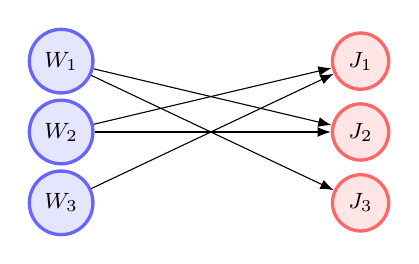
\begin{tikzpicture}[
        W/.style={circle, draw=blue!60, fill=blue!10, very thick, minimum size=5mm, font=\footnotesize},
        J/.style={circle, draw=red!60, fill=red!10, very thick, minimum size=5mm, font=\footnotesize},
        node distance=0.05cm and 3cm
    ]
    \node[W]      (w1)                     {$W_1$};
    \node[W]      (w2)       [below=of w1] {$W_2$};
    \node[W]      (w3)       [below=of w2] {$W_3$};

    \node[J]      (j1)       [right=of w1] {$J_1$};
    \node[J]      (j2)       [right=of w2] {$J_2$};
    \node[J]      (j3)       [right=of w3] {$J_3$};
     
    \draw[-Latex] (w1) -- (j2);
    \draw[-Latex] (w1) -- (j3);
    \draw[-Latex] (w2) -- (j1);
    \draw[-Latex] (w2) -- (j2);
    \draw[-Latex] (w3) -- (j1);
    \end{tikzpicture}
    \caption{Example of an instance of the bipartite matching problem.}
\end{figure}


\subsection{Maximum Cardinality Bipartite Matching}
The Maximum Cardinality Bipartite Matching problem consists on finding the maximum size bipartite matching in a given graph $G = (W, J, E)$. The objective is to find a matching such that the number of assignments is maximal.

\subsubsection{Reduction}
One way to solve this problem is to reduce it to the classical Max-Flow problem. We introduce two new nodes, $s$ and $t$; for each node $u \in W$ we add an edge $(s, u)$ and for each node $v \in J$ we add an edge $(v, t)$. The cardinality of the maximum matching is then the value of the max-flow from $s$ to $t$, and the matching itself consists of the edges used for the flow.

\begin{figure}[ht]
    \centering
    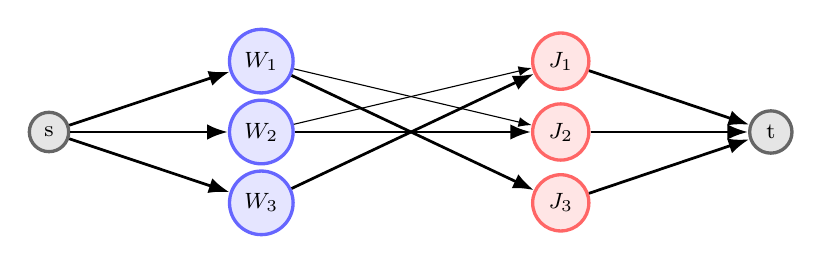
\begin{tikzpicture}[
        neutral/.style={circle, draw=black!60, fill=black!10, very thick, minimum size=5mm, font=\footnotesize},
        W/.style={circle, draw=blue!60, fill=blue!10, very thick, minimum size=5mm, font=\footnotesize},
        J/.style={circle, draw=red!60, fill=red!10, very thick, minimum size=5mm, font=\footnotesize},
        node distance=0.05cm and 3cm
    ]
    
    \node[W]       (w1)                     {$W_1$};
    \node[W]       (w2)       [below=of w1] {$W_2$};
    \node[W]       (w3)       [below=of w2] {$W_3$};
    \node[neutral] (s)        [left=2cm of w2]  {s};
    \node[J]       (j1)       [right=of w1] {$J_1$};
    \node[J]       (j2)       [right=of w2] {$J_2$};
    \node[J]       (j3)       [right=of w3] {$J_3$};
    \node[neutral] (t)        [right=2cm of j2] {t};
     
    \draw[-Latex, line width=0.35mm] (s) -- (w1);
    \draw[-Latex, line width=0.35mm] (s) -- (w2);
    \draw[-Latex, line width=0.35mm] (s) -- (w3);
    \draw[-Latex] (w1) -- (j2);
    \draw[-Latex, line width=0.35mm] (w1) -- (j3);
    \draw[-Latex] (w2) -- (j1);
    \draw[-Latex, line width=0.35mm] (w2) -- (j2);
    \draw[-Latex, line width=0.35mm] (w3) -- (j1);
    \draw[-Latex, line width=0.35mm] (j1) -- (t);
    \draw[-Latex, line width=0.35mm] (j2) -- (t);
    \draw[-Latex, line width=0.35mm] (j3) -- (t);
    \end{tikzpicture}
    \caption{Example of the reduction to Max-Flow, with the optimal solution marked in bold.}
\end{figure}

\subsubsection{Solution} \label{dinic}
One possible algorithm to solve the Max-Flow problem is Dinitz’ Algorithm which runs in $O(\left|V\right|^2 \left|E\right|)$ time \cite{schrijver_combinatorial_2013}. In practice, however, when using it to solve bipartite matching problems, the algorithm runs much faster; in fact it can be seen as a simplified form of the Hopcroft–Karp algorithm, which runs in time $O(\left|E\right|\sqrt{\left|V\right|})$ \cite{schrijver_combinatorial_2013}. The algorithm uses $O(\left|V\right| + \left|E\right|)$ memory.

Furthermore, for the case of maximum cardinality bipartite matching all weights are unitary and it is unnecessary to explicitly represent the flow.

\subsection{Maximum Weight Bipartite Matching}
Let us now consider the weighted version of the Maximum Bipartite Matching problem. Consider a graph $G = (W, J, E)$ and a function $r : E \mapsto \mathbb{R}$. As before the problem consists of selecting a subset of $E$ subject to each worker having at most one job, and each job being worked by at most one person. The goal is now to optimise this subset, $X \subset E$, such that $\sum_{x \in X} r(x)$ is maximal.

This problem is the maximisation version of the Assignment Problem\cite{korte_combinatorial_2012}.

\begin{figure}[ht]
    \centering
    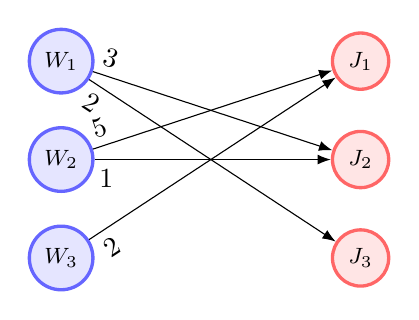
\begin{tikzpicture}[
        W/.style={circle, draw=blue!60, fill=blue!10, very thick, minimum size=5mm, font=\footnotesize},
        J/.style={circle, draw=red!60, fill=red!10, very thick, minimum size=5mm, font=\footnotesize},
        node distance=0.4cm and 3cm
    ]
    \node[W]      (w1)                     {$W_1$};
    \node[W]      (w2)       [below=of w1] {$W_2$};
    \node[W]      (w3)       [below=of w2] {$W_3$};

    \node[J]      (j1)       [right=of w1] {$J_1$};
    \node[J]      (j2)       [right=of w2] {$J_2$};
    \node[J]      (j3)       [right=of w3] {$J_3$};
     
    \draw[-Latex] (w1) -- node[pos=0.05, sloped, above] {3} (j2);
    \draw[-Latex] (w1) -- node[pos=0.05, sloped, below] {2} (j3);
    \draw[-Latex] (w2) -- node[pos=0.05, sloped, above] {5} (j1);
    \draw[-Latex] (w2) -- node[pos=0.05, sloped, below] {1} (j2);
    \draw[-Latex] (w3) -- node[pos=0.05, sloped, below] {2} (j1);
    \end{tikzpicture}
    \caption{Example of an instance of the weighted bipartite matching problem.} \label{wightex}
\end{figure}

\subsubsection{Reduction}
In order to use this algorithm we need to convert our problem to a minimisation problem. This can be done by creating a new $r$ function, $r'$ such that:
\[r'(e) = \max_{e' \in E}(r(e')) - r(e), \forall e \in E.\]

Moreover, the input to the problem is classically provided in matrix form: in tables~\ref{tab1}~and~\ref{tab2} we can see the original and transformed matrix, respectively, corresponding to the example in figure~\ref{wightex}.

\begin{table}[ht]
    \parbox{.45\linewidth}{
        \centering
        \begin{tabular}{cccc}
                  & $J_1$ & $J_2$ & $J_3$ \\
            $W_1$ & 0     & 3     & 2     \\
            $W_2$ & 5     & 1     & 0     \\
            $W_3$ & 2     & 0     & 0     \\
        \end{tabular}
        \caption{Original matrix, $r$.} \label{tab1}
    }
    \hfill
    \parbox{.45\linewidth}{
        \centering
        \begin{tabular}{cccc}
                  & $J_1$ & $J_2$ & $J_3$ \\
            $W_1$ & 5     & 2     & 3     \\
            $W_2$ & 0     & 4     & 5     \\
            $W_3$ & 3     & 5     & 5     \\
        \end{tabular}
        \caption{Modified matrix, $r'$.} \label{tab2}
    }
\end{table}

\subsubsection{Solution} \label{munkres}
A possible algorithm to solve the Assignment Problem is the Munkres Algorithm (also known as the \textit{Hungarian method} and several other names) \cite{schrijver_combinatorial_2013}. The algorithm starts with an empty matching, then it successively finds ``augmenting paths" such that a new matching with greater value is obtained. The algorithm as described by \textcite{jin_kue_wong_new_1979} runs in time $O(\left|V\right|^3)$. As for memory, the algorithm uses several auxiliary matrices/buffers amounting to $O(\left|V\right|^2)$.

\subsection{Matroids}
A matroid $M$ is a pair $(E, \mathcal{F})$, where $E$ is a a set (called the ground set) and $\mathcal{F}$ is a family of \textit{independent} subsets of $E$, subject to the following restrictions:
\begin{itemize}
    \setlength\itemsep{-.1em}
    \item $ \emptyset \in \mathcal{F} $,
    \item if $X \in \mathcal{F}$ and $Y \subseteq X$, then $Y \in \mathcal{F}$,
    \item if $X, Y \in \mathcal{F}$ and $|X| < |Y|$, then there is $y \in Y$ such that $X \cup \{y\} \in \mathcal{F}$.
\end{itemize}

\subsubsection{Matroid Intersection}
Let $M_1 = (S, \mathcal{F}_1)$ and $M_2 = (S, \mathcal{F}_2)$ be two matroids, on the same ground set $S$.
Then $\mathcal{F}_1 \cap \mathcal{F}_2$ corresponds to the common independent sets of both matroids, ie. their intersection.

The algorithm for computing the intersection of 2 matroids, as defined by \textcite{schrijver_combinatorial_2013}, can be shown to run in $O(n^2 m (n + Q))$ time (although better bounds have been found \cite{schrijver_combinatorial_2013}), where $n$ is the maximum size of a common independent set, $m$ is the size of the ground set, and $Q$ is the running time of the oracle \cite{schrijver_combinatorial_2013}. By analysing the algorithm we conclude that the spacial complexity is $O(m^2 + Q)$, where $Q$ is the spacial complexity of the oracle, resulting from constructing the bipartite graph $D_{M_1, M_2}(I)$.

If there are weights associated with the elements of the ground set, then the algorithm can be modified so that the maximum weight independent set is found instead.

\subsubsection{Bipartite Matching as a Matroid Problem}
Consider again the problem of bipartite matching in a graph $G = (W, J, E)$, where $V = W \cup J$.
Let $\delta : V \mapsto 2^E$ represent the edges incident on a given vertex, $v \in V$. Let also:

\begin{itemize}
    \setlength\itemsep{-.1em}
    \item $\mathcal{F}_W = \{X \subseteq E: |X \cap \delta(v)| \le 1, \forall v \in W\}$
    \item $\mathcal{F}_J = \{X \subseteq E: |X \cap \delta(v)| \le 1, \forall v \in J\}$
\end{itemize}

Then $M_W = (E, \mathcal{F}_W)$ and $M_J = (E, \mathcal{F}_J)$ are matroids \cite{goemans_handout_2011} (known as partition matroids). Furthermore, the largest cardinality element in the intersection corresponds to a maximum matching in G. If instead of the maximum cardinality, the objective was to obtain the maximum weight matching, then it would simply be needed to find the maximum total weight independent set, instead of the largest set possible.

The independence oracle for this matroid can be implemented in $O(1)$ time and $O(\left|V\right|)$ space, just by keeping a counter for each vertex representing the number of incident edges.

\subsubsection{r-Arborescences as a Matroid Problem}
Consider a directed graph $D = (V, E)$ and a special root vertex, $r \in V$. Then an r-arborescence is a directed spanning tree oriented away from $r$. We assume that graph $D$ has no incoming arcs into vertex $r$.

Let $G$ be the undirected counterpart of graph $D$. Note that if graph $D$ already contains edges $(u, v)$ and $(v, u)$ then they will also be duplicated in graph $G$. Let also:

\begin{itemize}
    \setlength\itemsep{-.1em}
    \item $\mathcal{F}_1 = \{X \subseteq E: \text{acyclic}(X)\}$,
    \item $\mathcal{F}_2 = \{X \subseteq E: |X \cap \delta^-(v)| \le 1, \forall v \in V \setminus \{r\} \}$,
\end{itemize}

where $\delta^-(v)$ corresponds to the set of edges incoming to $v$.

Then $M_1 = (E, \mathcal{F}_1)$ and $M_2 = (E, \mathcal{F}_2)$ are matroids (a graphic matroid and a partition matroid, respectively) \cite{goemans_handout_2011}. Moreover their intersection is the set of all sets of edges that are acyclic and where each vertex has at most one incoming edge, ie. an arborescence; maximising the cardinality of these sets makes it so that all paths must start in $r$ resulting in an r-arborescence.

A simple way to check independence of a given set is to just check if the corresponding graph is acyclic, using for example a DFS, resulting in $O(\left|V\right| + \left|E\right|)$.

\section{Implementation Details}
\subsection{Dinitz' Algorithm}
As mentioned in section~\ref{dinic} when solving maximum cardinality bipartite matching the flow on a given edge is always either one or zero, and as such it is possible to avoid representing the flow and the residual capacity. Moreover, if we modify the original graph to represent the residual capacity, then the algorithm needs no extra memory.

\subsection{Munkres Algorithm}
It is important to point out that we assumed our input graphs to be dense, which is why we chose the Munkres algorithm to solve this problem. If, however, the graphs were mostly sparse there would be two possible solutions:
\begin{itemize}
    \setlength\itemsep{-.1em}
    \item Modify the algorithm to use a sparse matrix. This however comes with a lot of problems as we need to ensure that the cells needed at each time step are \textit{active} in the matrix.
    \item Reduce the problem to min-cost max-flow, and use a different algorithm altogether.
\end{itemize}

The version of the Munkres algorithm we implemented is the one described by \textcite{r._a._pilgrim_munkres_nodate}, although we optimised a few cycles, particularly in step 4.

\subsection{Matroid Intersection Algorithm}
We created a generic \texttt{Matroid} class which includes the matroid intersection algorithm. Creating new kinds of matroids consists of creating subclasses and implementing the oracles.

It is also worth to mention that our Matroid interface requires two functions for the oracle, which allow for much faster oracle calls for some matroids:
\begin{itemize}
    \setlength\itemsep{-.1em}
    \item \texttt{is\_independent\_with(e)}$: E \mapsto $ \texttt{bool}\\
          This function checks if adding element \texttt{e} to the current independent set maintains independence or not;
    \item \texttt{is\_independent\_except\_with(e1, e2)}$: E \times E \mapsto $ \texttt{bool}\\
          This function checks if by removing element \texttt{e1} and adding \texttt{e2}, the current set is still independent.
\end{itemize}

\section{Experimental Analysis}
In this section each data point corresponds to the average of 11 executions of different problems generated with the same parameters. We also present in red the regression of the execution time and memory usage plots with respect to the theoretical complexities (note: to simplify the computation of the regressions we assumed the worst case of $\left|E\right| = \left|V\right|^2$).

Considering we used Python to implement our algorithms memory usage data might not be relevant, as it is a garbage collected language, nevertheless we present the results.

\subsection{Maximum Cardinality Bipartite Matching} \label{rmbm}
Explanation of the parameters:
\begin{itemize}
    \setlength\itemsep{-.1em}
    \item $p$: probability of a given edge $(w,j)$ existing;
    \item size: number of elements on each partition.
\end{itemize}

From the analysis of figure~\ref{bmr1} we can see that the running time of the algorithm seems to fit within the theoretical bounds (as stated in section \ref{dinic}). Moreover the space complexity also seems to fit the excepted behaviour.

Complementary, by analysing figure~\ref{bmr2} we can see that both time and spatial complexities are linear in the number of edges (when fixing the number of vertices), as would be expected.

\begin{figure}[ht]
\begin{subfigure}[b]{0.5\textwidth}
    \centering
    \begin{tikzpicture}
    	\begin{axis}[
    		perf,
    		title={Execution time for graphs with $p=0.1$},
    		xlabel={Size},
    		ylabel={Time [s]}
    		]
    		\addplot+[smooth, discard if not={p}{0.1}] table [x=s, y=t] {./card_matching.data};
    		\addplot+[red, no markers, domain=\pgfplotsxmin:\pgfplotsxmax, samples=20] {0.0295692946 -0.0000678864*x -0.0000096668*x^2 + 0.0000012287*x^(5/2)};
    	\end{axis}
    \end{tikzpicture}
\end{subfigure}%
\begin{subfigure}[b]{0.5\textwidth}
    \centering
    \begin{tikzpicture}
    	\begin{axis}[
    		perf,
    		title={Memory usage for graphs with $p=0.1$},
    		xlabel={Size},
    		ylabel={Memory [Kbytes]}
    		]
    		\addplot+[smooth, discard if not={p}{0.1}] table [x=s, y=mem] {./card_matching.data};
    		\addplot+[red, no markers, domain=\pgfplotsxmin:\pgfplotsxmax, samples=20] {9365.4935053571 +1.5611299039*x +0.0085201298*x^2};
    	\end{axis}
    \end{tikzpicture}
\end{subfigure}
\begin{subfigure}[b]{0.5\textwidth}
    \centering
    \begin{tikzpicture}
    	\begin{axis}[
    		perf,
    		title={Execution time for graphs with $p=1$},
    		xlabel={Size},
    		ylabel={Time [s]}
    		]
    		\addplot+[smooth, discard if not={p}{1}] table [x=s, y=t] {./card_matching.data};
    		\addplot+[red, no markers, domain=\pgfplotsxmin:\pgfplotsxmax, samples=20] {0.0253069607 +0.0046832076*x -0.0001635625*x^2 +0.0000153364*x^(5/2)};
    	\end{axis}
    \end{tikzpicture}
\end{subfigure}%
\begin{subfigure}[b]{0.5\textwidth}
    \centering
    \begin{tikzpicture}
    	\begin{axis}[
    		perf,
    		title={Memory usage for graphs with $p=1$},
    		xlabel={Size},
    		ylabel={Memory [Kbytes]}
    		]
    		\addplot+[smooth, discard if not={p}{1}] table [x=s, y=mem] {./card_matching.data};
    		\addplot+[red, no markers, domain=\pgfplotsxmin:\pgfplotsxmax, samples=20] {9328.1558464286 -1.8456623693*x +0.1081896105*x^2};
    	\end{axis}
    \end{tikzpicture}
\end{subfigure}
\caption{Execution results of the maximum cardinality bipartite matching problem.} \label{bmr1}
\end{figure}

\begin{figure}[ht]
\begin{subfigure}[b]{0.5\textwidth}
    \centering
	\begin{tikzpicture}
		\begin{axis}[
			perf,
			title={Execution time},
			xlabel={p},
			ylabel={Time [s]},
			legend to name=bmpleg,
			legend columns=3,
			legend style={font=\scriptsize}
			]
			\renewcommand{\do}[1]{
			    \addplot+[smooth, discard if not={s}{#1}] table [x=p, y=t] {./card_matching.data};
			    \addlegendentry{$#1$ nodes}
		    } \docsvlist{0,100,200,300,400,500}
		\end{axis}
	\end{tikzpicture}
\end{subfigure}%
\begin{subfigure}[b]{0.5\textwidth}
    \centering
	\begin{tikzpicture}
		\begin{axis}[
			perf,
			title={Memory usage},
			xlabel={p},
			ylabel={Memory [Kbytes]}
			]
			\renewcommand{\do}[1]{
			    \addplot+[smooth, discard if not={s}{#1}] table [x=p, y=mem] {./card_matching.data};
		    } \docsvlist{0,100,200,300,400,500}
		\end{axis}
	\end{tikzpicture}
\end{subfigure}

\begin{subfigure}[b]{\textwidth}
    \centering
	\ref{bmpleg}
\end{subfigure}
\caption{Evolution for different values of $p$ in the maximum cardinality bipartite matching problem.} \label{bmr2}
\end{figure}

\subsection{Maximum Weight Bipartite Matching}
Explanation of the parameters:
\begin{itemize}
    \setlength\itemsep{-.1em}
    \item $p$: probability of a given edge $(w,j)$ existing;
    \item $w$: maximum weight possible for any edge (weights follow a discrete uniform distribution~$\left]0, w\right]$);
    \item size: number of elements on each partition.
\end{itemize}

Looking at figures~\ref{wbmr1}~and~\ref{wbmr2} we conclude that the running time of this algorithm is also within the theoretical bounds (as stated in section \ref{munkres}). Furthermore the space complexity also corresponds to what was expected.

Figure~\ref{wbmr3} seems at first to be nonsensical, as the algorithm runs faster for problems with more edges. This is however because, as previously referred, the Hungarian method works best when graphs are dense.

As for the effect of the weights' magnitude, even though just by looking at figure~\ref{wbmr4} one might think that they do have an impact, this is actually because increasing the number of possible weight values, also increases the number of possible optimal solution values. If we were to change the magnitude of the weights uniformly (ie. multiplying all of them by some large number) we would see that it doesn't actually impact the performance of the algorithm, as would be expected. The differences in memory usage are because of the way Python handles small integer numbers.

\begin{figure}[ht]
\begin{subfigure}[b]{0.5\textwidth}
    \centering
	\begin{tikzpicture}
		\begin{axis}[
			perf,
			title={Execution time for graphs with $p=0.1$},
			xlabel={Size},
			ylabel={Time [s]}
			]
			\addplot+[smooth, discard if not={p}{0.1}, discard if not={w}{100}] table [x=s, y=t] {./weight_matching.data};
			\addplot+[red, no markers, domain=\pgfplotsxmin:\pgfplotsxmax, samples=20] {0.0694996031 -0.0060505581*x +0.0000900166*x^2 + 0.0000000408*x^3};
		\end{axis}
	\end{tikzpicture}
\end{subfigure}%
\begin{subfigure}[b]{0.5\textwidth}
    \centering
	\begin{tikzpicture}
		\begin{axis}[
			perf,
			title={Memory usage for graphs with $p=0.1$},
			xlabel={Size},
			ylabel={Memory [Kbytes]}
			]
			\addplot+[smooth, discard if not={p}{0.1}, discard if not={w}{100}] table [x=s, y=mem] {./weight_matching.data};
			\addplot+[red, no markers, domain=\pgfplotsxmin:\pgfplotsxmax, samples=20] {9546.8051921429 -1.0807272407*x +0.0320467532*x^2};
		\end{axis}
	\end{tikzpicture}
\end{subfigure}

\begin{subfigure}[b]{0.5\textwidth}
    \centering
    	\begin{tikzpicture}
		\begin{axis}[
			perf,
			title={Execution time for graphs with $p=1$},
			xlabel={Size},
			ylabel={Time [s]}
			]
			\addplot+[smooth, discard if not={p}{1}, discard if not={w}{100}] table [x=s, y=t] {./weight_matching.data};
			\addplot+[red, no markers, domain=\pgfplotsxmin:\pgfplotsxmax, samples=20] {0.0726992062 -0.0063962661*x +0.0000656417*x^2 -0.0000000488*x^3};
		\end{axis}
	\end{tikzpicture}
\end{subfigure}%
\begin{subfigure}[b]{0.5\textwidth}
    \centering
	\begin{tikzpicture}
		\begin{axis}[
			perf,
			title={Memory usage for graphs with $p=1$},
			xlabel={Size},
			ylabel={Memory [Kbytes]}
			]

			\addplot+[smooth, discard if not={p}{1}, discard if not={w}{100}] table [x=s, y=mem] {./weight_matching.data};
			\addplot+[red, no markers, domain=\pgfplotsxmin:\pgfplotsxmax, samples=20] {9436.7662332143 +0.7862207832*x +0.0864655844*x^2};
		\end{axis}
	\end{tikzpicture}
\end{subfigure}
\caption{Execution results of the maximum weight bipartite matching problem, with $w=100$.} \label{wbmr1}
\end{figure}

\begin{figure}[ht]
\begin{subfigure}[b]{0.5\textwidth}
    \centering
	\begin{tikzpicture}
		\begin{axis}[
			perf,
			title={Execution time for graphs with $p=0.1$},
			xlabel={Size},
			ylabel={Time [s]}
			]
			\addplot+[smooth, discard if not={p}{0.1}, discard if not={w}{5000}] table [x=s, y=t] {./weight_matching.data};
			\addplot+[red, no markers, domain=\pgfplotsxmin:\pgfplotsxmax, samples=20] {0.7175587288 -0.0744357749*x +0.0005522684*x^2 +0.0000001602*x^3};
		\end{axis}
	\end{tikzpicture}
\end{subfigure}%
\begin{subfigure}[b]{0.5\textwidth}
    \centering
	\begin{tikzpicture}
		\begin{axis}[
			perf,
			title={Memory usage for graphs with $p=0.1$},
			xlabel={Size},
			ylabel={Memory [Kbytes]}
			]
			\addplot+[smooth, discard if not={p}{0.1}, discard if not={w}{5000}] table [x=s, y=mem] {./weight_matching.data};
			\addplot+[red, no markers, domain=\pgfplotsxmin:\pgfplotsxmax, samples=20] {9507.8961003571 -0.0943895911*x +0.0567974026*x^2};
		\end{axis}
	\end{tikzpicture}
\end{subfigure}

\begin{subfigure}[b]{0.5\textwidth}
    \centering
    	\begin{tikzpicture}
		\begin{axis}[
			perf,
			title={Execution time for graphs with $p=1$},
			xlabel={Size},
			ylabel={Time [s]}
			]
			\addplot+[smooth, discard if not={p}{1}, discard if not={w}{5000}] table [x=s, y=t] {./weight_matching.data};
			\addplot+[red, no markers, domain=\pgfplotsxmin:\pgfplotsxmax, samples=20] {0.0222757935 -0.0090352779*x +0.0001582225*x^2 +0.0000000783*x^3};
		\end{axis}
	\end{tikzpicture}
\end{subfigure}%
\begin{subfigure}[b]{0.5\textwidth}
    \centering
	\begin{tikzpicture}
		\begin{axis}[
			perf,
			title={Memory usage for graphs with $p=1$},
			xlabel={Size},
			ylabel={Memory [Kbytes]}
			]
			\addplot+[smooth, discard if not={p}{1}, discard if not={w}{5000}] table [x=s, y=mem] {./weight_matching.data};
			\addplot+[red, no markers, domain=\pgfplotsxmin:\pgfplotsxmax, samples=20] {9335.8571428571 +1.2752337757*x +0.1122538961*x^2};
		\end{axis}
	\end{tikzpicture}
\end{subfigure}
\caption{Execution results of the maximum weight bipartite matching problem, with $w=5000$.} \label{wbmr2}
\end{figure}

\begin{figure}[ht]
\begin{subfigure}[b]{0.5\textwidth}
    \centering
	\begin{tikzpicture}
		\begin{axis}[
			perf,
			title={Execution time with $w = 100$},
			xlabel={p},
			ylabel={Time [s]}
			]
			\renewcommand{\do}[1]{
			    \addplot+[smooth, discard if not={s}{#1}, discard if not={w}{100}] table [x=p, y=t] {./weight_matching.data};
		    } \docsvlist{0,100,200,300,400,500}
		    
		\end{axis}
	\end{tikzpicture}
\end{subfigure}
\begin{subfigure}[b]{0.5\textwidth}
    \centering
	\begin{tikzpicture}
		\begin{axis}[
			perf,
			title={Memory usage with $w = 100$},
			xlabel={p},
			ylabel={Memory [Kbytes]}
			]
			\renewcommand{\do}[1]{
			    \addplot+[smooth, discard if not={s}{#1}, discard if not={w}{100}] table [x=p, y=mem] {./weight_matching.data};
		    } \docsvlist{0,100,200,300,400,500}
		    
		\end{axis}
	\end{tikzpicture}
\end{subfigure}

\begin{subfigure}[b]{0.5\textwidth}
    \centering
    \begin{tikzpicture}
    	\begin{axis}[
    		perf,
    		title={Execution time with $w = 5000$},
    		xlabel={p},
    		ylabel={Time [S]}
    		]
    		\renewcommand{\do}[1]{
    		    \addplot+[smooth, discard if not={s}{#1}, discard if not={w}{5000}] table [x=p, y=t] {./weight_matching.data};
    	    } \docsvlist{0,100,200,300,400,500}
    	\end{axis}
    \end{tikzpicture}
\end{subfigure}
\begin{subfigure}[b]{0.5\textwidth}
    \centering
    \begin{tikzpicture}
    	\begin{axis}[
    		perf,
    		title={Memory usage with $w = 5000$},
    		xlabel={p},
    		ylabel={Memory [Kbytes]}
    		]
    		\renewcommand{\do}[1]{
    		    \addplot+[smooth, discard if not={s}{#1}, discard if not={w}{5000}] table [x=p, y=mem] {./weight_matching.data};
    	    } \docsvlist{0,100,200,300,400,500}
    	\end{axis}
    \end{tikzpicture}
\end{subfigure}

\begin{subfigure}[b]{\textwidth}
    \centering
	\ref{bmpleg}
\end{subfigure}
\caption{Evolution for different values of $p$ in the maximum weight bipartite matching problem.} \label{wbmr3}
\end{figure}

\begin{figure}[ht]
\begin{subfigure}[b]{0.5\textwidth}
    \centering
	\begin{tikzpicture}
		\begin{axis}[
			perf,
			title={Execution time with $p = 0.1$},
			xlabel={w},
			ylabel={Time [s]}
			]
			\renewcommand{\do}[1]{
			    \addplot+[smooth, discard if not={s}{#1}, discard if not={p}{0.1}] table [x=w, y=t] {./weight_matching.data};
		    } \docsvlist{0,100,200,300,400,500}
		    
		\end{axis}
	\end{tikzpicture}
\end{subfigure}
\begin{subfigure}[b]{0.5\textwidth}
    \centering
	\begin{tikzpicture}
		\begin{axis}[
			perf,
			title={Memory usage with $p = 0.1$},
			xlabel={w},
			ylabel={Memory [Kbytes]}
			]
			\renewcommand{\do}[1]{
			    \addplot+[smooth, discard if not={s}{#1}, discard if not={p}{0.1}] table [x=w, y=mem] {./weight_matching.data};
		    } \docsvlist{0,100,200,300,400,500}
		    
		\end{axis}
	\end{tikzpicture}
\end{subfigure}

\begin{subfigure}[b]{0.5\textwidth}
    \centering
	\begin{tikzpicture}
		\begin{axis}[
			perf,
			title={Execution time with $p = 1$},
			xlabel={w},
			ylabel={Time [S]}
			]
			\renewcommand{\do}[1]{
			    \addplot+[smooth, discard if not={s}{#1}, discard if not={p}{1}] table [x=w, y=t] {./weight_matching.data};
		    } \docsvlist{0,100,200,300,400,500}
		\end{axis}
	\end{tikzpicture}
\end{subfigure}
\begin{subfigure}[b]{0.5\textwidth}
    \centering
	\begin{tikzpicture}
		\begin{axis}[
			perf,
			title={Memory usage with $p = 1$},
			xlabel={w},
			ylabel={Memory [Kbytes]}
			]
			\renewcommand{\do}[1]{
			    \addplot+[smooth, discard if not={s}{#1}, discard if not={p}{1}] table [x=w, y=mem] {./weight_matching.data};
		    } \docsvlist{0,100,200,300,400,500}
		\end{axis}
	\end{tikzpicture}
\end{subfigure}

\begin{subfigure}[b]{\textwidth}
    \centering
	\ref{bmpleg}
\end{subfigure}
\caption{Evolution for different values of $w$ in the maximum weight bipartite matching problem.} \label{wbmr4}
\end{figure}

\subsection{Matroid based Maximum Cardinality Bipartite Matching}
Explanation of the parameters:
\begin{itemize}
    \setlength\itemsep{-.1em}
    \item $p$: probability of a given edge $(w,j)$ existing;
    \item size: number of elements on each partition.
\end{itemize}

The first thing to notice when looking at figure~\ref{mbmr1} is that this algorithm is much slower than the max-flow reduction in section~\ref{rmbm}, however (assuming we already have a matroid intersection algorithm) there is almost nothing to implement: just the oracles.

As before, analysing figures~\ref{mbmr1}~and~\ref{mbmr2} leads us to believe that our algorithm fits the expected time and space requirements; in particular figure~\ref{mbmr2} indicates that the algorithm in linear in the number of edges, as was indicated by the theoretical bounds.

\begin{figure}[ht]
\begin{subfigure}[b]{0.5\textwidth}
    \centering
	\begin{tikzpicture}
		\begin{axis}[
			perf,
			title={Execution time for graphs with $p=0.1$},
			xlabel={Size},
			ylabel={Time [s]}
			]
			\addplot+[smooth, discard if not={p}{0.1}] table [x=s, y=t] {./matroid_matching.data};
			\addplot+[red, no markers, domain=\pgfplotsxmin:\pgfplotsxmax, samples=20] {0.0292153148 -0.0515979292*x +0.0048181597*x^2 -0.0001489192*x^3 +0.0000018470*x^4 -0.0000000052*x^5};
		\end{axis}
	\end{tikzpicture}
\end{subfigure}
\begin{subfigure}[b]{0.5\textwidth}
    \centering
	\begin{tikzpicture}
		\begin{axis}[
			perf,
			title={Memory usage for graphs with $p=0.1$},
			xlabel={Size},
			ylabel={Memory [Kbytes]}
			]

			\addplot+[smooth, discard if not={p}{0.1}] table [x=s, y=mem] {./matroid_matching.data};
			\addplot+[red, no markers, domain=\pgfplotsxmin:\pgfplotsxmax, samples=20] {9326.7902448699 +111.3245237783*x -6.0268663679*x^2 +0.1044058767*x^3 -0.0004329201*x^4};
		\end{axis}
	\end{tikzpicture}
\end{subfigure}
\begin{subfigure}[b]{0.5\textwidth}
    \centering
	\begin{tikzpicture}
		\begin{axis}[
			perf,
			title={Execution time for graphs with $p=1$},
			xlabel={Size},
			ylabel={Time [s]}
			]
			\addplot+[smooth, discard if not={p}{1}] table [x=s, y=t] {./matroid_matching.data};
			\addplot+[red, no markers, domain=\pgfplotsxmin:\pgfplotsxmax, samples=20] {0.2172006615 -1.5015912645*x +0.1275467114*x^2 -0.0034975469*x^3 +0.0000386399*x^4 -0.0000001191*x^5};
		\end{axis}
	\end{tikzpicture}
\end{subfigure}
\begin{subfigure}[b]{0.5\textwidth}
    \centering
	\begin{tikzpicture}
		\begin{axis}[
			perf,
			title={Memory usage for graphs with $p=1$},
			xlabel={Size},
			ylabel={Memory [Kbytes]}
			]
			\addplot+[smooth, discard if not={p}{1}] table [x=s, y=mem] {./matroid_matching.data};
			\addplot+[red, no markers, domain=\pgfplotsxmin:\pgfplotsxmax, samples=20] {9433.9149900499 -78.1198928825*x +6.5447279281*x^2 -0.0251456608*x^3 +0.0006276429*x^4};
		\end{axis}
	\end{tikzpicture}
\end{subfigure}
\caption{Execution results of the matroid maximum cardinality bipartite matching problem.} \label{mbmr1}
\end{figure}

\begin{figure}[ht]
\begin{subfigure}[b]{0.5\textwidth}
    \centering
	\begin{tikzpicture}
		\begin{axis}[
			perf,
			title={Evolution for different $p$},
			xlabel={p},
			ylabel={Time [s]},
			legend to name=mbmpleg,
			legend columns=4,
			legend style={font=\scriptsize}
			]
			\renewcommand{\do}[1]{
			    \addplot+[smooth, discard if not={s}{#1}] table [x=p, y=t] {./matroid_matching.data};
			    \addlegendentry{$#1$ nodes}
		    } \docsvlist{0,20,40,60,80,100,120}
		\end{axis}
	\end{tikzpicture}
\end{subfigure}
\begin{subfigure}[b]{0.5\textwidth}
	\begin{tikzpicture}
		\begin{axis}[
			perf,
			title={Evolution for different $p$},
			xlabel={p},
			ylabel={Memory [Kbytes]}
			]
			\renewcommand{\do}[1]{
			    \addplot+[smooth, discard if not={s}{#1}] table [x=p, y=mem] {./matroid_matching.data};
		    } \docsvlist{0,20,40,60,80,100,120}
		\end{axis}
	\end{tikzpicture}
\end{subfigure}

\begin{subfigure}[b]{\textwidth}
    \centering
	\ref{mbmpleg}
\end{subfigure}
\caption{Evolution for different values of $p$ in the matroid maximum cardinality bipartite matching problem.} \label{mbmr2}
\end{figure}

\subsection{Matroid r-Arborescences}
Explanation of the parameters:
\begin{itemize}
    \setlength\itemsep{-.1em}
    \item $p$: probability of a given edge $(u,v)$ existing;
    \item size: number of elements on each partition.
\end{itemize}

The first thing to notice when observing figure~\ref{arbr1} is that the number of instances has been cut down from the previous problem, in particular when the graph is dense we actually had to stop the computation because it was taking too long. We see that for $p = 1$ the interpolation of our data points is above the obtained regression but theorise that it is because the data has too little resolution compared to the rate of growth of the running time.

In figure~\ref{arbr2} we were expecting to see a non-linearity because of the running time of the oracle being $O(\left|V\right| + \left|E\right|)$, which would result in the time being quadratic with respect to $\left|E\right|$. However from the little data points obtained the algorithm appears to still be linear on the number of edges; this might be because although a DFS depends linearly on both the number of vertices and edges, particular applications might be more sensitive to one or the other. %TODO CHECK THIS -> probably not true

\begin{figure}[ht]
\begin{subfigure}[b]{0.5\textwidth}
    \centering
	\begin{tikzpicture}
		\begin{axis}[
			perf,
			title={Execution time for graphs with $p=0.1$},
			xlabel={Size},
			ylabel={Time [s]}
			]
			\addplot+[smooth, discard if not={p}{0.1}] table [x=s, y=t] {./matroid_arborescence.data};
			\addplot+[red, no markers, domain=\pgfplotsxmin:\pgfplotsxmax, samples=20] {-0.0117647109 +0.4216356982*x -0.0497746995*x^2 +0.0019716567*x^3 -0.0000344823*x^4 +0.0000003128*x^5};
		\end{axis}
	\end{tikzpicture}
\end{subfigure}
\begin{subfigure}[b]{0.5\textwidth}
    \centering
	\begin{tikzpicture}
		\begin{axis}[
			perf,
			title={Memory usage for graphs with $p=0.1$},
			xlabel={Size},
			ylabel={Memory [Kbytes]}
			]

			\addplot+[smooth, discard if not={p}{0.1}] table [x=s, y=mem] {./matroid_arborescence.data};
			\addplot+[red, no markers, domain=\pgfplotsxmin:\pgfplotsxmax, samples=20] {9352.0794970129 +73.3388419241*x -5.4722007418*x^2 +0.1318836845*x^3 -0.0007102404*x^4};
		\end{axis}
	\end{tikzpicture}
\end{subfigure}
\begin{subfigure}[b]{0.5\textwidth}
    \centering
	\begin{tikzpicture}
		\begin{axis}[
			perf,
			title={Execution time for graphs with $p=1$},
			xlabel={Size},
			ylabel={Time [s]}
			]
			\addplot+[smooth, discard if not={p}{1}] table [x=s, y=t] {./matroid_arborescence.data};
			\addplot+[red, no markers, domain=\pgfplotsxmin:\pgfplotsxmax, samples=20] {0.0245500000 -0.0066984229*x -0.0479549684*x^2 +0.0058603796*x^3 -0.0002163551*x^4 +0.0000033700*x^5};
		\end{axis}
	\end{tikzpicture}
\end{subfigure}
\begin{subfigure}[b]{0.5\textwidth}
    \centering
	\begin{tikzpicture}
		\begin{axis}[
			perf,
			title={Memory usage for graphs with $p=1$},
			xlabel={Size},
			ylabel={Memory [Kbytes]}
			]
			\addplot+[smooth, discard if not={p}{1}] table [x=s, y=mem] {./matroid_arborescence.data};
			\addplot+[red, no markers, domain=\pgfplotsxmin:\pgfplotsxmax, samples=20] {9426.5454499642 +114.5333317842*x -15.0158920931*x^2 +0.7518922514*x^3 -0.0061049008*x^4};
		\end{axis}
	\end{tikzpicture}
\end{subfigure}
\caption{Execution results of the matroid r-arborescence problem.} \label{arbr1}
\end{figure}

\begin{figure}[ht]
\begin{subfigure}[b]{0.5\textwidth}
    \centering
	\begin{tikzpicture}
		\begin{axis}[
			perf,
			title={Evolution for different $p$},
			xlabel={p},
			ylabel={Time [s]},
			legend to name=arbpleg,
			legend columns=4,
			legend style={font=\scriptsize}
			]
			\renewcommand{\do}[1]{
			    \addplot+[smooth, discard if not={s}{#1}] table [x=p, y=t] {./matroid_arborescence.data};
			    \addlegendentry{$#1$ nodes}
		    } \docsvlist{0,15,30,45,60,75,90}
		\end{axis}
	\end{tikzpicture}
\end{subfigure}
\begin{subfigure}[b]{0.5\textwidth}
	\begin{tikzpicture}
		\begin{axis}[
			perf,
			title={Evolution for different $p$},
			xlabel={p},
			ylabel={Memory [Kbytes]}
			]
			\renewcommand{\do}[1]{
			    \addplot+[smooth, discard if not={s}{#1}] table [x=p, y=mem] {./matroid_arborescence.data};
		    } \docsvlist{0,15,30,45,60,75,90}
		\end{axis}
	\end{tikzpicture}
\end{subfigure}

\begin{subfigure}[b]{\textwidth}
    \centering
	\ref{arbpleg}
\end{subfigure}
\caption{Evolution for different values of $p$ in the matroid r-arborescence problem.} \label{arbr2}
\end{figure}

\renewcommand*{\bibfont}{\footnotesize}
\small
\printbibliography
\end{document}
